\documentclass[12pt,a4paper]{article}
\usepackage{amsmath}
\usepackage{amssymb}  % Provides \mathbb and other symbols
\usepackage{graphicx}
\usepackage{subcaption}
\usepackage{enumitem}
\usepackage{listings}
\usepackage{hyperref}
\usepackage{ulem}
\usepackage{xcolor}
\usepackage{amsthm}
\usepackage{tcolorbox}  % For colored boxes
\usepackage[table]{xcolor} % For coloring table cells
\usepackage{array}         % For better table alignment
\usepackage{mdframed}
\usepackage{cancel}
\usepackage[margin=2.5cm]{geometry}
\setlength{\parindent}{0pt}
\setlength{\parskip}{0.8em}

\begin{document}
\begin{titlepage}
\centering
\vspace*{\fill}
{\Huge Analysis III} \\[0.5cm]
{\Huge Home Work 1}\\[1.5cm]
{\Large Student: 26-712-224}\\[0.5cm]
{\Large \today}
\vspace*{\fill}
\end{titlepage}

\newpage
\section*{Exercise 1 (Analysis II Recap, 1+1+1 P.)}
Let $I=[a;b]$ be a compact interval in $\mathbb{R}$.
\begin{enumerate}[label=(\alph*)]
\item Explain the following statement: ``The inclusion
\begin{align*}
T(I,\mathbb{R}) \subseteq S(I,\mathbb{R})
\end{align*}
is dense with respect to the supremum-norm.'' In particular, define the spaces $T(I,\mathbb{R})$ and $S(I,\mathbb{R})$ and the supremum-norm. (See Chapters 6 and 7 in the script.)
\item Explain briefly how the above can be used to define the (Riemann) integral
\begin{align*}
\int_a^b f(x)dx
\end{align*}
for any $f\in S(I,\mathbb{R})$.
\item Construct a sequence of functions in $T(I,\mathbb{R})$ converging uniformly to $f(x)=x$ on $I=[0;1]$. (You do not have to prove the uniform convergence.)
\end{enumerate}
ANSWER:\\
(a) In the Analysis II notes:
\begin{itemize}
    \item $T(I, \mathbb{R})$ is defined to be the \textbf{set of step functions} with domain I - a (perfect) interval of $\bar{\mathbb{R}}$ - and 
whose co-domain is $\mathbb{R}$.
    \item $S(I, \mathbb{R})$ is defined as the set of \textbf{regulated functions} - ie functions, $f:I \to \mathbb{R}$, which have both right and 
left hand limits $\forall x \in I$ and these limits are finite.
    \item The supremum-norm is defined on all bounded function $f: I \to \mathbb{R}$ as given by: $||f||_{\infty} = \sup_{x \in I}||f(x)||$; where, 
    in this case, I have chosen the absolute value norm on $\mathbb{R}$
\end{itemize}
The "Inclusion" statement means that, using the supremum-norm, any "regulated function" can be approximated to by step functions with any degree
of accuracy.\\
\\
(b) As $T(I, \mathbb{R})$ is dense in $S(I, \mathbb{R})$ we know that given any $\epsilon > 0$, we can find a sequence $(f_k)_{k \in \mathbb{N}}$ of
step function in $T(I, \mathbb{R})$ which converges using the supremum norm to $f \in S(I, \mathbb{R})$.  That is:
\begin{align*}
 \|f-f_k\|_{\infty}<\epsilon \;\;\;\;\;\;\;\;\;\;\;\;\;\; \forall k > N \;\;\; (N \in \mathbb{N})
\end{align*}
Under such conditions we could then define the Riemann integral of $f \in S(I, \mathbb{R})$ by:
\begin{align*}
\int_a^b f = \lim_{k \to \infty} \int_a^b f_k \;\;\;\;\;\;\;\;\; \text{(where I = [a,b])}
\end{align*}
\newpage
\noindent
(c) Firstly, we divide $[0,1]$ into $k$ evenly spaced intervals: $[0 = \frac{0}{k}, \frac{1}{k}, \frac{2}{k}, ..., \frac{k-1}{k}, 1=\frac{k}{k}]$. \\
Now let us create the sequence of step functions $(f_k)_{k \in \mathbb{N}}$, where each $f_k \in T([0, 1], \mathbb{R})$, that converge uniformly 
to $f(x)=x$ on $[0,1]$:
\begin{align*}
 f_k(x) = \frac{j}{k} \;\;\;\;\;\;\;\;\;\;\;\; \text{when $x \in \left[\frac{j}{k}, \frac{j+1}{k}\right)$ and $f_k(1)=1$}
\end{align*}

\newpage
\section*{Exercise 2 (Null sets, 3+4 P.)}
In this exercise we show that two sets are Lebesgue null.
\begin{enumerate}[label=(\alph*)]
\item Let $N=\mathbb{R}^{n-1}\times\{0\}\subset\mathbb{R}^n$. Using a similar strategy as in Example 11.1.4 (3) in the script, show that $N$ is a set of measure zero.
\item Denote by
\begin{align*}
S^1=\{x\in\mathbb{R}^2:|x|=1\}
\end{align*}
the unit circle in $\mathbb{R}^2$. For $m\in\mathbb{N}$, take $x_1,\ldots,x_m$ to be $m$ equidistantly placed points on $S^1$. Using squares of equal sizes centered at these points and eventually sending $m\to+\infty$, show that $S^1$ is a set of measure zero.

\textit{Hint:} How large must these squares be so that they cover the circle? You may use without proof that the distance between two points on $S^1$ is at most as large as the angle between them.
\end{enumerate}
ANSWER:\\
(a) $N=R^{(n-1)} \times \{0\}$ and we now wish to show that this set in $R^n$ has measure zero.\\
\\
I will use a slightly different strategy than in Example 11.1.4 (3) - which I find simpler.\\
\\
Given $\epsilon > 0$ consider the sequence of \textbf{open} and \textbf{bounded} intervals:
$$U_m := (-m, m) \times (-m, m) \times ... \times (-m, m) \times (-\frac{\epsilon}{2^{m+1}(2m)^{(n-1)}}, \frac{\epsilon}{2^{m+1}(2m)^{(n-1)}}) $$
where there are $(n-1)$ terms of the form $(-m, m)$.  Then it is clear that we have an open cover for $N$:
\begin{align*}
N \subset \bigcup_{m=1}^{\infty} U_m \tag{2.1}
\end{align*}
We can easily compute the Lebesgue measure for each $U_m$ as:
\begin{align*}
\lambda_n (U_m) = (2m)^{(n-1)} \frac{\epsilon}{2^m(2m)^{(n-1)}} = \frac{\epsilon}{2^m} \tag{2.2}
\end{align*}
From (2.1) and (2.2) we conclude that:
\begin{align*}
\lambda_n (N) &\le \sum_{m=1}^{\infty} \lambda_n(U_m) \\
  &\le \sum_{m=1}^{\infty} \frac{\epsilon}{2^m} \\
  &\le \epsilon
\end{align*}
As $\epsilon$ is arbitatrary we can conclude that $N$ is a set of measure zero (in $\mathbb{R}^n$).

\newpage
\noindent
(b) We will denote the set of points that comprise the boundary of the unit circle $S^1$ by $\partial S$.\\
\\
Consider the diagram below showing the $m$ points $p_1, p_2,..., p_m$ that are equally spaced on the circumference of the circle.
\begin{figure}[h]
\centering
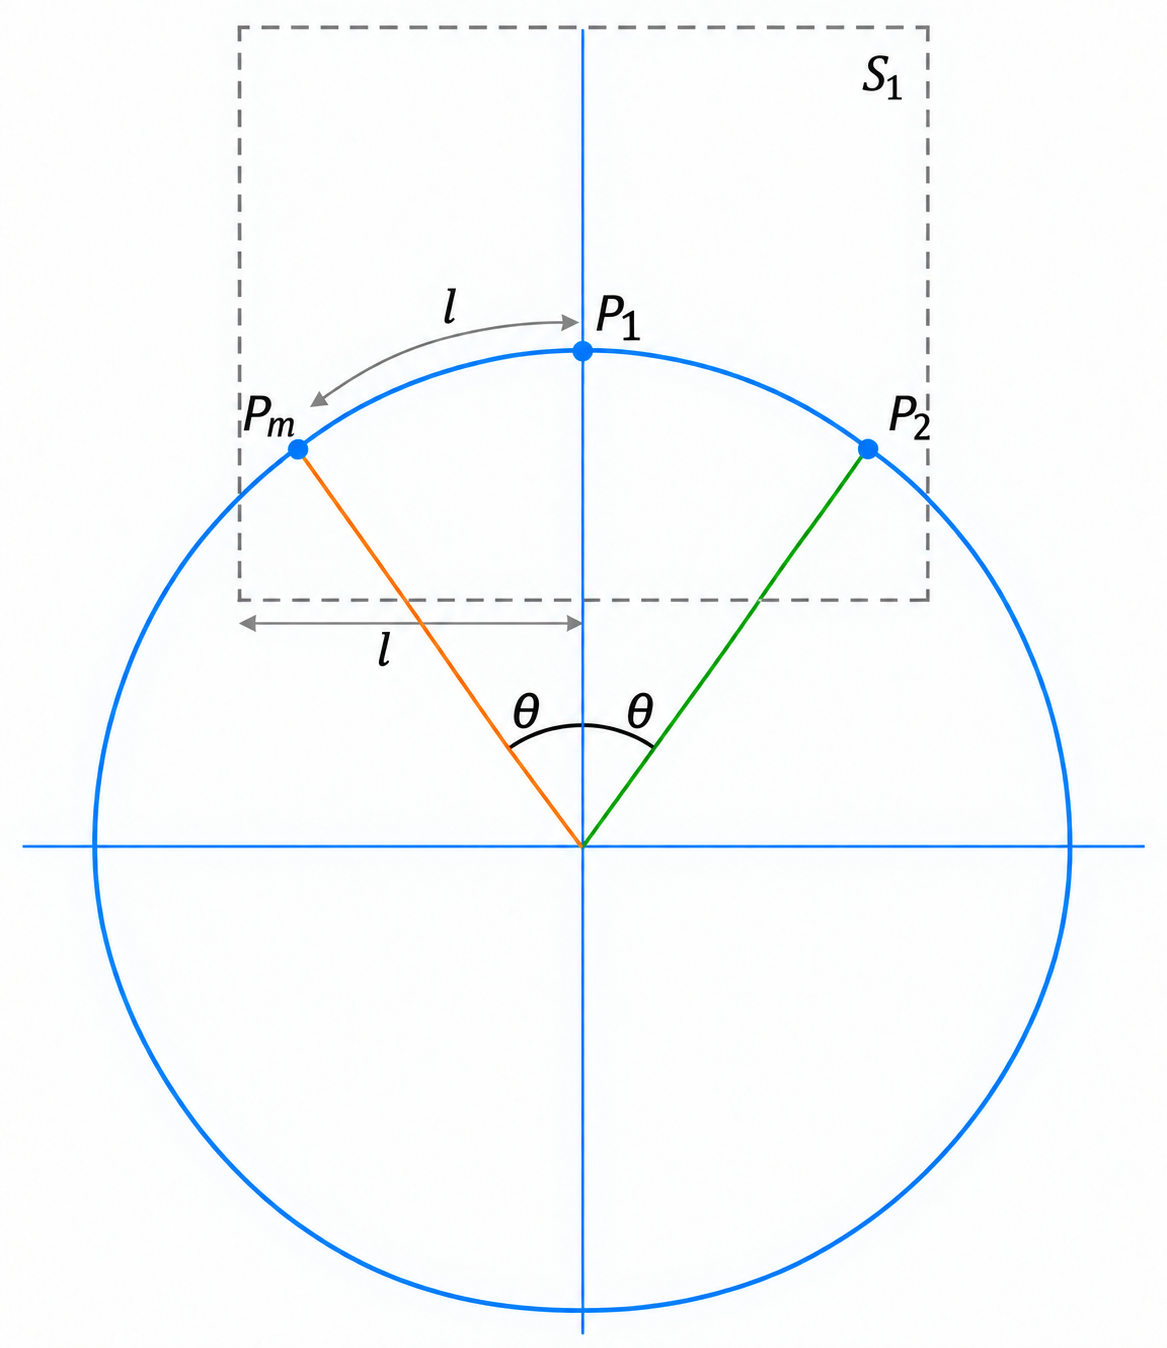
\includegraphics[width=0.7\textwidth]{Diagrams/ANAL_III_WK_1_Q2.png}
\caption{Circle construction}
\end{figure}
The angle, extended from the centre of the circle, to each consecutive point on the circumference is $\theta = \frac{2 \pi}{m}$.  This means that, on the unit circle, the 
length of the arc between consecutive points is: $l = \frac{2 \pi}{m}$.\\
Taking the point $p_i$ as the centre of an \textbf{open} square of side length $2l =  \frac{4 \pi}{m}$, we can refer to this open square as $S_i$ - An example of $S_1$ 
is shown in the diagram (but $p_1$ is a little "off centre" due to limitations of drawing).\\
\\
It should be clear that the Lebesgue measure (i.e. area) of each such square is: $\lambda_2(S_i) = (2l)^2 = \frac{16 \pi^2}{m^2}$.\\
\\
The $m$ squares $(S_i)_{i=1}^m$ - which are each \textbf{open} and \textbf{bounded} - overlap and completely cover the boundary, $\partial S$.  Hence:
\begin{align*}
\partial S \subset \bigcup_{i=1}^{m} S_i \tag{2.3}
\end{align*}
Hence, we can obtain an upper bound for the Lebesgue measure for the set $\partial S$ from:
\begin{align*}
\lambda_2 (\partial S) &\le \sum_{i=1}^{m} \lambda_2(S_i) \\
  &\le \sum_{m=1}^m \frac{16 \pi^2}{m^2} \\
  &\le \frac{16 \pi^2}{m} \tag{2.4}
\end{align*}
Given any $\epsilon > 0$ we can find an integer $M \in \mathbb{N}$ such that $M > \frac{16 \pi^2}{\epsilon}$ for which (2.4) is smaller then $\epsilon$, whenever $m > M$,
and we can conclude that, in $\mathbb{R}^2$, the set $\partial S$ has measure zero.

\newpage
\section*{Exercise 5 (Jordan null sets)}
Let $A\subset\mathbb{R}^n$. We say that $A$ is a \textit{Jordan null set} if for any $\varepsilon>0$ there exist finitely many $(n$-dimensional) open intervals $I_1,\ldots,I_m$ with the property
\begin{align*}
\sum_{k=1}^{m}\lambda_n(I_k)<\varepsilon
\qquad\text{and}\qquad
A\subset\bigcup_{k=1}^{m}I_k.
\end{align*}
Observe that by definition every Jordan null set is also Lebesgue null.
\begin{enumerate}[label=(\alph*)]
\item Show that any Jordan null set is necessarily bounded.
\item Give an example of an uncountable Jordan null set in $\mathbb{R}^2$.
\item Give an example of a Lebesgue null set in $\mathbb{R}$ that is \textit{not} a Jordan null set.
\end{enumerate}
Answer:\\
(a) Each interval in $(I_k)_{k=1}^m$ is bounded and this means that their (finite) union must also be bounded.\\
Indeed, let $I_k = (a_{k,1}, b_{k,1}) \times (a_{k,2}, b_{k,2}) \times ... \times (a_{k,n}, b_{k,n})$, then it is clear that in each of the
$n$ dimensions we can create: $a_i = min_k(a_{k,i})$ and $b_i = max_k(a_{k,i})$.  Then it is clear that:
\begin{align*}
 &I_k \subset (a_1, b_1) \times (a_2, b_2) \times ... \times (a_n, b_n) \;\;\;\;\;\;\;\;\;\;\;\;\;\;\; \forall k = 1,2,...,m \\
 \implies &A \subset \bigcup_{i=1}^m I_k \subset (a_1, b_1) \times (a_2, b_2) \times ... \times (a_n, b_n)
\end{align*}
\qed\\
\\
(b) Consider the set: $S = (0,1) \times \{0\}$ - it is definitely uncountable.  Given $\epsilon > 0$, we can then consider the single open covering:
\begin{align*}
   I_1 = (0,1) \times (-\epsilon/3, \epsilon/3)
\end{align*}
Clearly $S \subset I_1$ and $\lambda_2(I_1) = (1-0) \frac{2}{3}\epsilon < \epsilon$.  Hence, the set $S$ is a Jordan null set.\\
\\
(c) As Jordan null sets are always bounded we can easily find a Lebesgue null set that is not a Jordan null set.\\
Consider the set $\mathbb{N}$ - which is an \textbf{unbounded} countable collection of points - i.e. a countable collection of null sets
and hence is a Lebesgue null set, but NOT a Jordan null set.

\end{document}